\documentclass[11pt]{article}

\usepackage[letterpaper,margin=0.88in]{geometry}
\usepackage[T1]{fontenc}
\usepackage{lmodern}
\usepackage{microtype}
\usepackage{amsmath,amssymb,mathtools}
\usepackage{bm}
\usepackage{booktabs}
\usepackage{array}
\usepackage{enumitem}
\usepackage{xcolor}
\usepackage{tikz}
\usetikzlibrary{arrows.meta,positioning,calc,decorations.pathreplacing}
\usepackage{caption}
\usepackage[colorlinks=true,linkcolor=blue!45!black,citecolor=blue!45!black,urlcolor=blue!45!black,pdftitle={Butterfly factorization through invariants},pdfsubject={Middle-seeded butterfly factorization and a target-only alternative},pdfkeywords={butterfly factorization, invariant, complementary low rank, target-only factorization}]{hyperref}

\setlength{\parskip}{0.35em}
\setlength{\parindent}{0pt}
\setlist{itemsep=0.25em,topsep=0.35em}
\captionsetup{font=small,labelfont=bf,width=0.94\textwidth}
\allowdisplaybreaks[1]

\definecolor{sourceblue}{RGB}{34,94,153}
\definecolor{targetred}{RGB}{166,67,54}
\definecolor{softblue}{RGB}{219,233,246}
\definecolor{softred}{RGB}{247,226,220}
\definecolor{softgreen}{RGB}{224,240,229}
\definecolor{gridgray}{RGB}{177,184,190}

\newcommand{\C}{\mathbb{C}}
\newcommand{\e}{\varepsilon}
\newcommand{\jd}{\bar\jmath}
\newcommand{\given}{\,|\,}
\newcommand{\simeqeps}{\simeq_{\e}}
\DeclareMathOperator{\range}{range}
\DeclareMathOperator{\diag}{diag}
\DeclareMathOperator{\Spans}{span}

\tikzset{
  grid16/.pic={
    \foreach \g in {0,...,16} {
      \draw[gridgray,line width=0.22pt] (\g*0.16,0) -- (\g*0.16,-2.56);
      \draw[gridgray,line width=0.22pt] (0,-\g*0.16) -- (2.56,-\g*0.16);
    }
    \draw[black,line width=0.65pt] (0,0) rectangle (2.56,-2.56);
  },
  stage/.style={draw,rounded corners=2pt,align=center,text width=2.18cm,minimum height=1.52cm,font=\scriptsize,inner sep=4pt},
  source/.style={stage,fill=softblue,draw=sourceblue},
  target/.style={stage,fill=softred,draw=targetred},
  flow/.style={-{Latex[length=2mm]},thick},
  construction/.style={draw,rounded corners=2pt,align=center,text width=3.35cm,minimum height=1.25cm,font=\scriptsize,inner sep=5pt,fill=black!3}
}

\title{\textbf{Butterfly factorization through invariants}\\[0.3em]
\large The middle-seeded algorithm and a target-only alternative}
\author{}
\date{}

\begin{document}
\maketitle

\begin{abstract}
A butterfly factorization applies a complementary-low-rank matrix through a sequence of small local operations.  This report explains the method using invariants: statements about the intermediate data that remain true from one level to the next.  The original construction of Li et al. has two online invariants, one for compressed input bands and one for compressed output contributions, joined at the middle level.  The middle is an \emph{offline} construction device: balanced blocks minimize the generic sampling cost before any input vector exists.  A different, middle-seeded construction instead gives every online vector the same partial-product meaning.  Its coarse factors are obtained by small QR factorizations, without accessing the original matrix again.  The supplied implementation of this target-only form was correct to roundoff in the reported tests and slightly faster, with the same asymptotic complexity.  We then carry the same invariant over to interpolative decomposition butterfly factorization (IDBF).  A new controlled local-ID prototype implements IDBF's two-sided organization and its target-only counterpart from shared middle data.  Both are correct to roundoff in the reported tests; the target-only application has lower measured runtime and storage.  Construction measurements are explicitly limited to this visible-entry mathematical-oracle prototype, rather than the paper's optimized sampled-entry constructor.
\end{abstract}

\tableofcontents

\section{What an algorithm invariant is}

An \textbf{invariant} is a property of an algorithm's state that is true at a specified point in its execution and remains true whenever the algorithm advances.  A useful invariant answers three questions at once: what the intermediate data mean, why one update is valid, and why the final state solves the problem.

For example, let $a=(2,-1,5,4)$ and consider
\[
 s\gets0;\qquad \text{for }t=0,1,2,3:\quad s\gets s+a_t .
\]
At the start of iteration $t$, with zero-based indexing, the invariant is
\[
 \boxed{\;s=\sum_{q=0}^{t-1}a_q\;}.
\]
It holds initially because $s=0$ is the empty sum.  Adding $a_t$ preserves it with $t$ replaced by $t+1$.  On termination, $t=4$, so $s=\sum_{q=0}^{3}a_q=10$.  The first four states below are checked before the update; the last is the output:
\begin{center}
\begin{tabular}{c|ccccc}
\toprule
$t$ & 0 & 1 & 2 & 3 & 4\\
$s$ & 0 & 2 & 1 & 6 & 10\\
sum already read & $()$ & $(2)$ & $(2,-1)$ & $(2,-1,5)$ & $(2,-1,5,4)$\\
\bottomrule
\end{tabular}
\end{center}
The butterfly invariants have exactly the same logical role, but their state is an indexed collection of short vectors rather than one scalar.

\section{Complementary blocks and the low-rank hypothesis}
\label{sec:blocks}

\subsection{One indexing system for the whole report}

Let $K\in\C^{N\times N}$ with $N=2^L$, and let $g\in\C^N$.  We seek $u=Kg$.  Rows and columns use the indices $0,\dots,N-1$.  A dyadic interval at depth $d$ is
\[
 D_i^d:=\{iN/2^d,\dots,(i+1)N/2^d-1\},\qquad 0\le i<2^d .
\]
Let $A_i^\ell=D_i^\ell$ be a \emph{row node} and $B_j^{L-\ell}=D_j^{L-\ell}$ a \emph{column node} at the complementary depth.  Define the block and input band
\[
 K_{ij}^{\ell}:=K[A_i^\ell,B_j^{L-\ell}]
 \in\C^{(N/2^\ell)\times 2^\ell},
 \qquad g_j^\ell:=g[B_j^{L-\ell}],
 \tag{1}\label{eq:block}
\]
where $0\le i<2^\ell$ and $0\le j<2^{L-\ell}$.  The pair $(i,j)$ is a \textbf{slot}.  There are $2^\ell2^{L-\ell}=N$ slots, and their blocks tile $K$.  Increasing $\ell$ splits every row node in two and merges two column nodes.

All matrix figures use $N=16$, hence $L=4$ and middle level $h=2$.  We write $a:b=\{a,\dots,b-1\}$; end indices are excluded.  Thus ``rows $8:12$'' means rows $8,9,10,11$.

\begin{figure}[htbp]
\centering
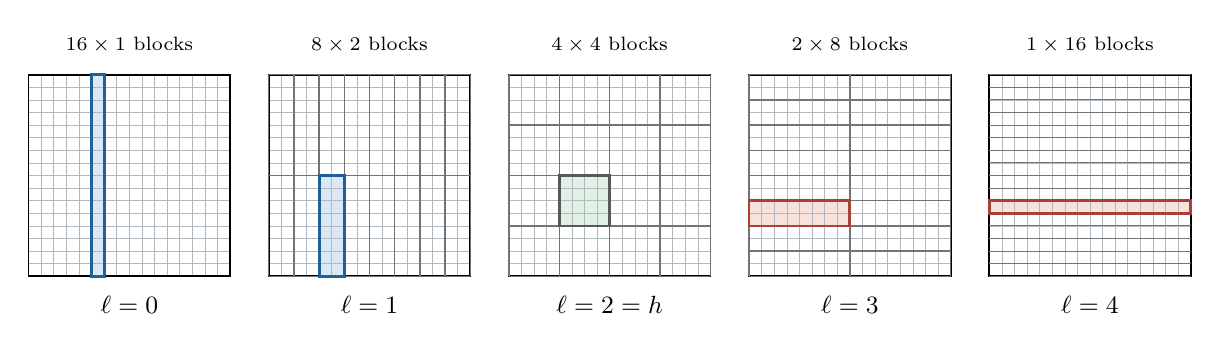
\begin{tikzpicture}[x=1cm,y=1cm]
% Level 0: slot (0,5) = all rows, column 5.
\begin{scope}[shift={(0,0)}]
  \fill[softblue] (5*.16,0) rectangle (6*.16,-2.56);
  \pic {grid16};
  \draw[sourceblue,line width=1pt] (5*.16,0) rectangle (6*.16,-2.56);
  \node[font=\scriptsize] at (1.28,0.38) {$16\times1$ blocks};
  \node[font=\small] at (1.28,-2.92) {$\ell=0$};
\end{scope}
% Level 1: slot (1,2) = rows 8:16, columns 4:6.
\begin{scope}[shift={(3.05,0)}]
  \fill[softblue] (4*.16,-8*.16) rectangle (6*.16,-16*.16);
  \pic {grid16};
  \foreach \g in {0,...,8}{\draw[black!55,line width=.5pt] (\g*.32,0)--(\g*.32,-2.56);}
  \draw[black!55,line width=.5pt] (0,0)--(2.56,0) (0,-1.28)--(2.56,-1.28) (0,-2.56)--(2.56,-2.56);
  \draw[sourceblue,line width=1pt] (4*.16,-8*.16) rectangle (6*.16,-16*.16);
  \node[font=\scriptsize] at (1.28,0.38) {$8\times2$ blocks};
  \node[font=\small] at (1.28,-2.92) {$\ell=1$};
\end{scope}
% Level 2: slot (2,1) = rows 8:12, columns 4:8.
\begin{scope}[shift={(6.10,0)}]
  \fill[softgreen] (4*.16,-8*.16) rectangle (8*.16,-12*.16);
  \pic {grid16};
  \foreach \g in {0,...,4}{\draw[black!55,line width=.5pt] (\g*.64,0)--(\g*.64,-2.56) (0,-\g*.64)--(2.56,-\g*.64);}
  \draw[black!65,line width=1pt] (4*.16,-8*.16) rectangle (8*.16,-12*.16);
  \node[font=\scriptsize] at (1.28,0.38) {$4\times4$ blocks};
  \node[font=\small] at (1.28,-2.92) {$\ell=2=h$};
\end{scope}
% Level 3: slot (5,0) = rows 10:12, columns 0:8.
\begin{scope}[shift={(9.15,0)}]
  \fill[softred] (0,-10*.16) rectangle (8*.16,-12*.16);
  \pic {grid16};
  \foreach \g in {0,...,8}{\draw[black!55,line width=.5pt] (0,-\g*.32)--(2.56,-\g*.32);}
  \draw[black!55,line width=.5pt] (0,0)--(0,-2.56) (1.28,0)--(1.28,-2.56) (2.56,0)--(2.56,-2.56);
  \draw[targetred,line width=1pt] (0,-10*.16) rectangle (8*.16,-12*.16);
  \node[font=\scriptsize] at (1.28,0.38) {$2\times8$ blocks};
  \node[font=\small] at (1.28,-2.92) {$\ell=3$};
\end{scope}
% Level 4: slot (10,0) = row 10, all columns.
\begin{scope}[shift={(12.20,0)}]
  \fill[softred] (0,-10*.16) rectangle (2.56,-11*.16);
  \pic {grid16};
  \foreach \g in {0,...,16}{\draw[black!55,line width=.4pt] (0,-\g*.16)--(2.56,-\g*.16);}
  \draw[targetred,line width=1pt] (0,-10*.16) rectangle (2.56,-11*.16);
  \node[font=\scriptsize] at (1.28,0.38) {$1\times16$ blocks};
  \node[font=\small] at (1.28,-2.92) {$\ell=4$};
\end{scope}
\end{tikzpicture}
\caption{The five complementary tilings of a $16\times16$ matrix.  Every panel has exactly $16$ equal-area blocks; only block boundaries are emphasized.  The outlined blocks are, from left to right, $K_{0,5}^0=K[0:16,5:6]$, $K_{1,2}^1=K[8:16,4:6]$, $K_{2,1}^2=K[8:12,4:8]$, $K_{5,0}^3=K[10:12,0:8]$, and $K_{10,0}^4=K[10:11,0:16]$.  These are actual slots in the tiling, not arbitrary rectangles.}
\label{fig:tilings}
\end{figure}

\subsection{The required structure is local, not global}

A \textbf{truncated singular value decomposition} (SVD) will be our standard local approximation.  If $Z\in\C^{m\times n}$, a retained rank $\rho$ gives
\[
 Z\simeqeps P C Q^*,\qquad P^*P=Q^*Q=I_\rho,
\]
where $P\in\C^{m\times\rho}$ is an output (column-space) basis, $Q\in\C^{n\times\rho}$ is an input (row-space) basis, and $C\in\C^{\rho\times\rho}$.  For a truncated SVD, $C=\Sigma$ is diagonal with retained singular values and $\|Z-PCQ^*\|_2$ is the first discarded singular value.  The star denotes conjugate transpose.  More generally, an approximate SVD or another low-rank factorization can be used.

The sole structural assumption is the following:
\begin{quote}
\textbf{Complementary low-rank property.}  For every level $\ell$ and every slot, $K_{ij}^{\ell}$ has numerical rank at most $r$ at the requested tolerance $\e$.  That is, a rank-$(\le r)$ approximation has error bounded by $\e$, in the local metric chosen by the construction.
\end{quote}
This does \emph{not} require the whole matrix $K$ to have rank $r$.  Full columns ($\ell=0$) and full rows ($\ell=L$) are automatically rank one; balanced blocks are the substantial low-rank requirement.  Fourier and Fourier-integral matrices are standard examples in which complementary, rather than global, low rank is useful \cite{BF,IDBF}.

The effective coordinate count is capped by the block dimensions:
\[
 \rho_\ell\le\min\{r,N/2^\ell,2^\ell\}.
 \tag{2}\label{eq:rho}
\]
For $N=16$ and $r\ge4$, one can take $(\rho_0,\dots,\rho_4)=(1,2,4,2,1)$.  Consequently, a level containing one short vector per slot has at most $N\rho_\ell\le Nr$ coefficients.

The approximation signs below include low-rank truncations.  Restricting to row children and adding contributions over disjoint column bands are exact operations.  This distinction is essential to the invariant proofs.

\section{The original butterfly factorization: two invariants}
\label{sec:original}

\subsection{Why construction starts in the middle}
\label{sec:why-middle}

The original factorization of Li et al. \cite{BF} is
\[
 K\approx U^L G^{L-1}\cdots G^h M^h(H^h)^*\cdots(H^{L-1})^*(V^L)^*,
 \qquad h=L/2 .
 \tag{3}\label{eq:bf-product}
\]
For our $16\times16$ example it reads $K\approx U^4G^3G^2M^2(H^2)^*(H^3)^*(V^4)^*$.  Its construction starts with all middle blocks:
\[
 K_{ij}^{h}\simeqeps P_{ij}^{h}C_{ij}^{h}(Q_{ij}^{h})^* .
 \tag{4}\label{eq:middle-seed}
\]
The factorization \eqref{eq:bf-product} is then built by recursive local compressions away from this seed.

\begin{center}
\fcolorbox{black!35}{black!4}{\parbox{0.94\textwidth}{
\textbf{The reason for the middle is offline complexity.}  Construction happens once, before any particular $g$ is supplied and before any application $Kg$ has been performed.  The balanced seed minimizes the generic cost of obtaining local low-rank information; it is not an extra online approximation principle.
}}
\end{center}

To see the balance, fix a level $\ell$.  Its $N$ blocks have dimensions $(N/2^\ell)\times2^\ell$.  Sampling $O(\rho_\ell)$ rows and columns of every block costs, up to the local decomposition constants,
\[
 O\!\left(N\rho_\ell\left(\frac{N}{2^\ell}+2^\ell\right)\right)
 \tag{5}\label{eq:sampling-cost}
\]
entry accesses.  At fixed rank, $N/2^\ell+2^\ell$ is minimized when $2^\ell=\sqrt N$, namely at $\ell=h$.  The middle-seeded entry-sampling construction therefore has the paper's $O(N^{3/2})$ order under its randomized-sampling and incoherence assumptions.  If fast black-box products by $K$ and $K^*$ are available instead, the corresponding middle-seed term is $O(N^{1/2}C_K(N))$, where $C_K(N)$ is the cost of one such product \cite{BF}.

By contrast, starting a direct orthonormal target construction at $\ell=0$ requires normalized full columns.  Their $N^2$ entries, and even all exact column norms, require $\Theta(N^2)$ entry accesses in the worst case.  This is an obstruction to \emph{direct construction}, not to applying a diagonal factor once it has been built.  Section~\ref{sec:target-only} shows how the middle seed avoids that obstruction while removing the middle hand-off from the final online factors.

We use orthonormal $P,Q$ and a small coupling $C$ for clarity.  The paper moves diagonal singular-value scalings into its block factors; diagonal rescaling converts between these normalizations.

\subsection{Invariant I: compressed input bands (the source half)}
\label{sec:source-invariant}

During application, let $t$ denote the \emph{actual block level}, increasing from $0$ to $h$ on the source half.  This avoids confusing block level with the paper's decreasing factor superscript $\ell=L-t$.  The source state at level $t$ is one vector $z_{ij}^{t}\in\C^{\rho_t}$ per slot, satisfying
\[
 \boxed{\quad z_{ij}^{t}\approx(Q_{ij}^{t})^*g_j^t,\qquad0\le t\le h. \quad}
 \tag{6}\label{eq:source-invariant}
\]
At $t=0$, each band is one input entry and $Q_{0j}^0$ is a $1\times1$ basis, so $z_{0j}^0$ is $g_j$ up to a unit-modulus scalar.  The diagonal factor $(V^L)^*$ performs this initialization in the present normalization.

For an update from $t-1$ to $t$, choose a destination $(i',j')$ and put $i=\lfloor i'/2\rfloor$.  Its two parent slots are $a=(i,2j')$ and $b=(i,2j'+1)$.  Since the new band is the disjoint concatenation of the old bands,
\[
 F_{i'j'}^{t}:=(Q_{i'j'}^{t})^*
 \begin{bmatrix}Q_a^{t-1}&0\\0&Q_b^{t-1}\end{bmatrix},
 \qquad
 z_{i'j'}^{t}=F_{i'j'}^{t}
 \begin{bmatrix}z_a^{t-1}\\z_b^{t-1}\end{bmatrix} .
 \tag{7}\label{eq:source-update}
\]
The local matrix has size $\rho_t\times(\rho_a+\rho_b)$.  The complementary low-rank property, applied to row spaces (equivalently, to column spaces of $K^*$), keeps this change of input basis short.  The matrices $F$ are the local blocks of the source factors $(H^\ell)^*$ after global slot ordering is included.

Equation \eqref{eq:source-invariant} is the first original invariant: the slots contain \emph{coordinates of the input}, not yet pieces of the output.

\subsection{The middle hand-off}

At $t=h$, equations \eqref{eq:middle-seed} and \eqref{eq:source-invariant} give
\[
 P_{ij}^{h}C_{ij}^{h}z_{ij}^{h}
 =P_{ij}^{h}C_{ij}^{h}(Q_{ij}^{h})^*g_j^h
 \approx K_{ij}^{h}g_j^h .
\]
Thus the state becomes an output partial product by setting
\[
 w_{ij}^{h}:=C_{ij}^{h}z_{ij}^{h}.
 \tag{8}\label{eq:hand-off}
\]
The sparse matrix $M^h$ applies these local couplings and reorders slots between source-friendly and target-friendly layouts.  It does not combine different matrix blocks.  For an SVD seed, $C$ is diagonal and this stage costs only $O(N\rho_h)$ arithmetic operations.

\subsection{Invariant II: compressed output contributions (the target half)}

For every level $t$, the second kind of state is defined by
\[
 \boxed{\quad P_{ij}^{t}w_{ij}^{t}\approx K_{ij}^{t}g_j^t. \quad}
 \tag{9}\label{eq:target-invariant}
\]
The left side is a short-coordinate representation of one block applied to one input band.  For fixed $i$, summing these vectors over $j$ gives the approximate answer on the rows $A_i^t$.  Equation \eqref{eq:hand-off} establishes this invariant at $t=h$.

\begin{figure}[htbp]
\centering
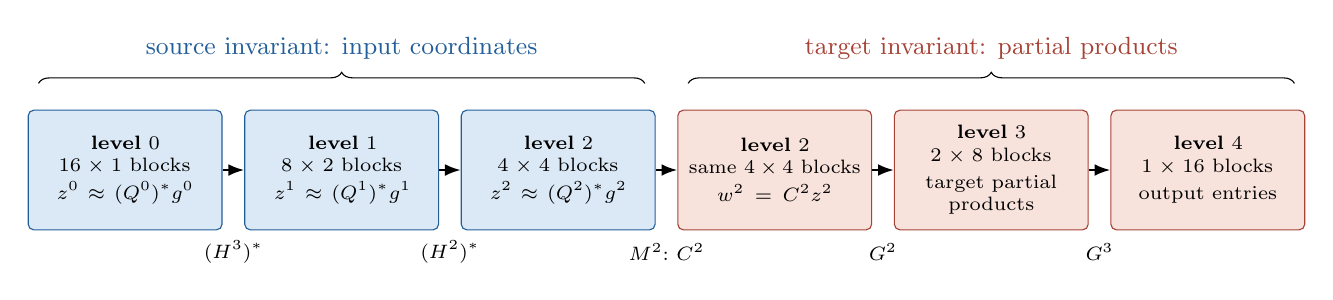
\begin{tikzpicture}[x=1cm,y=1cm]
\node[source] (z0) at (0,0) {\textbf{level $0$}\\$16\times1$ blocks\\[2pt]$z^0\approx(Q^0)^*g^0$};
\node[source] (z1) at (2.75,0) {\textbf{level $1$}\\$8\times2$ blocks\\[2pt]$z^1\approx(Q^1)^*g^1$};
\node[source] (z2) at (5.50,0) {\textbf{level $2$}\\$4\times4$ blocks\\[2pt]$z^2\approx(Q^2)^*g^2$};
\node[target] (w2) at (8.25,0) {\textbf{level $2$}\\same $4\times4$ blocks\\[2pt]$w^2=C^2z^2$};
\node[target] (w3) at (11.0,0) {\textbf{level $3$}\\$2\times8$ blocks\\[2pt]target partial products};
\node[target] (w4) at (13.75,0) {\textbf{level $4$}\\$1\times16$ blocks\\[2pt]output entries};
\draw[flow] (z0)--(z1); \node[font=\scriptsize] at ($(z0)!0.5!(z1)+(0,-1.04)$) {$(H^3)^*$};
\draw[flow] (z1)--(z2); \node[font=\scriptsize] at ($(z1)!0.5!(z2)+(0,-1.04)$) {$(H^2)^*$};
\draw[flow] (z2)--(w2); \node[font=\scriptsize] at ($(z2)!0.5!(w2)+(0,-1.04)$) {$M^2$:\ $C^2$};
\draw[flow] (w2)--(w3); \node[font=\scriptsize] at ($(w2)!0.5!(w3)+(0,-1.04)$) {$G^2$};
\draw[flow] (w3)--(w4); \node[font=\scriptsize] at ($(w3)!0.5!(w4)+(0,-1.04)$) {$G^3$};
\draw[decorate,decoration={brace,amplitude=4pt}] (-1.1,1.10)--(6.60,1.10);
\node[font=\small,text=sourceblue] at (2.75,1.55) {source invariant: input coordinates};
\draw[decorate,decoration={brace,amplitude=4pt}] (7.15,1.10)--(14.85,1.10);
\node[font=\small,text=targetred] at (11.0,1.55) {target invariant: partial products};
\end{tikzpicture}
\caption{The original online sweep for $N=16$.  Initialization by $(V^4)^*$ and terminal scaling by $U^4$ are scalar operations on singleton bases.  Source levels advance from $0$ to $2$; $M^2$ changes the meaning of the state without changing the block level; target levels then advance from $2$ to $4$.  There are two invariants, not one.}
\label{fig:original-pipeline}
\end{figure}

\subsection{One geometric step: two matrices become two matrices}
\label{sec:target-update}

The target update is easiest to understand at the matrix level.  Consider level $\ell+1$, a destination slot $(i',j')$, and $i=\lfloor i'/2\rfloor$.  With $a=(i,2j')$ and $b=(i,2j'+1)$, restriction $R_{i'}$ to the row child gives the exact identity
\[
 K_{i'j'}^{\ell+1}
 =R_{i'}\begin{bmatrix}K_a^\ell&K_b^\ell\end{bmatrix}.
 \tag{10}\label{eq:block-split}
\]
Each of the two old matrices is read by \emph{both} row children.  Hence a whole level takes two parent matrices and produces two child matrices, as Figure~\ref{fig:two-two} illustrates with actual $16\times16$ indices.  It is not a global two-to-one reduction.

\begin{figure}[htbp]
\centering
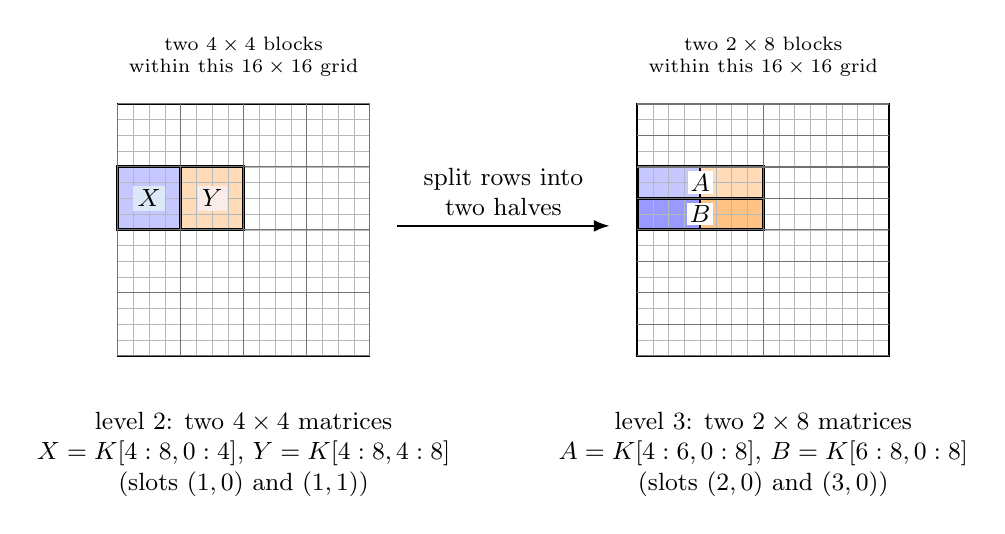
\begin{tikzpicture}[x=1cm,y=1cm]
% Parent level 2: the two 4x4 matrices X=K[4:8,0:4], Y=K[4:8,4:8].
\begin{scope}[shift={(0,0)},scale=1.25]
  \fill[blue!22] (0,-4*.16) rectangle (4*.16,-8*.16);
  \fill[orange!28] (4*.16,-4*.16) rectangle (8*.16,-8*.16);
  \pic[transform shape] {grid16};
  \draw[line width=1pt] (0,-4*.16) rectangle (4*.16,-8*.16);
  \draw[line width=1pt] (4*.16,-4*.16) rectangle (8*.16,-8*.16);
  \foreach \g in {0,...,4} {
    \draw[black!55,line width=.45pt] (\g*.64,0)--(\g*.64,-2.56);
    \draw[black!55,line width=.45pt] (0,-\g*.64)--(2.56,-\g*.64);
  }
  \node[font=\small,fill=softblue,inner sep=1.5pt] at (2*.16,-6*.16) {$X$};
  \node[font=\small,fill=softred!65!white,inner sep=1.5pt] at (6*.16,-6*.16) {$Y$};
  \node[font=\scriptsize,align=center] at (1.28,0.48) {two $4\times4$ blocks\\within this $16\times16$ grid};
\end{scope}
\node[align=center,font=\small] at (1.6,-4.45) {level $2$: two $4\times4$ matrices\\$X=K[4:8,0:4]$, $Y=K[4:8,4:8]$\\(slots $(1,0)$ and $(1,1)$)};
\draw[flow] (3.55,-1.55)--node[above,align=center,font=\small]{split rows into\\two halves}(6.25,-1.55);
% Child level 3: top/bottom 2x8 matrices with the blocks again inside the grid.
\begin{scope}[shift={(6.6,0)},scale=1.25]
  \fill[blue!22] (0,-4*.16) rectangle (4*.16,-6*.16);
  \fill[orange!28] (4*.16,-4*.16) rectangle (8*.16,-6*.16);
  \fill[blue!40] (0,-6*.16) rectangle (4*.16,-8*.16);
  \fill[orange!48] (4*.16,-6*.16) rectangle (8*.16,-8*.16);
  \pic[transform shape] {grid16};
  \draw[line width=1pt] (0,-4*.16) rectangle (8*.16,-6*.16);
  \draw[line width=1pt] (0,-6*.16) rectangle (8*.16,-8*.16);
  \draw[line width=.7pt] (4*.16,-4*.16)--(4*.16,-8*.16);
  \foreach \g in {0,...,8}{\draw[black!55,line width=.5pt] (0,-\g*.32)--(2.56,-\g*.32);}
  \draw[black!55,line width=.5pt] (1.28,0)--(1.28,-2.56);
  \node[font=\small,fill=white,inner sep=1pt] at (4*.16,-5*.16) {$A$};
  \node[font=\small,fill=white,inner sep=1pt] at (4*.16,-7*.16) {$B$};
  \node[font=\scriptsize,align=center] at (1.28,0.48) {two $2\times8$ blocks\\within this $16\times16$ grid};
\end{scope}
\node[align=center,font=\small] at (8.2,-4.45) {level $3$: two $2\times8$ matrices\\$A=K[4:6,0:8]$, $B=K[6:8,0:8]$\\(slots $(2,0)$ and $(3,0)$)};
\end{tikzpicture}
\caption{Two matrices in, two matrices out, for the middle step $\ell=2\to3$.  Here $X$ and $Y$ occupy adjacent $4\times4$ blocks inside the $16\times16$ matrix.  Split both at rows $4:6$ and $6:8$.  If $R_{\mathrm t}$ and $R_{\mathrm b}$ select those two row sets, $A=R_{\mathrm t}[X\ Y]$ and $B=R_{\mathrm b}[X\ Y]$.  All highlighted blocks stay inside the $16\times16$ grid and track exactly these row/column sets.}
\label{fig:two-two}
\end{figure}

At the vector level, suppose the target invariant holds at level $\ell$.  Define the small transfer
\[
 G_{i'j'}^{\ell}:=(P_{i'j'}^{\ell+1})^*
 \begin{bmatrix}R_{i'}P_a^\ell&R_{i'}P_b^\ell\end{bmatrix}
 \in\C^{\rho_{\ell+1}\times(\rho_a+\rho_b)}
 \tag{11}\label{eq:G-definition}
\]
The online vector update derived from this matrix step is
\[
 \boxed{\quad w_{i'j'}^{\ell+1}=G_{i'j'}^{\ell}
 \begin{bmatrix}w_a^\ell\\w_b^\ell\end{bmatrix}.\quad}
 \tag{12}\label{eq:target-update}
\]
This one multiplication implements three conceptual operations: restrict the old outputs to a row child, add the two column-band contributions, and project into the new output basis.

To verify preservation, let $\Pi_{i'j'}^{\ell+1}=P_{i'j'}^{\ell+1}(P_{i'j'}^{\ell+1})^*$.  Substitution gives
\[
\begin{aligned}
 P_{i'j'}^{\ell+1}w_{i'j'}^{\ell+1}
 &=\Pi_{i'j'}^{\ell+1}R_{i'}(P_a^\ell w_a^\ell+P_b^\ell w_b^\ell)\\
 &\approx\Pi_{i'j'}^{\ell+1}R_{i'}(K_a^\ell g_a^\ell+K_b^\ell g_b^\ell)
 =\Pi_{i'j'}^{\ell+1}K_{i'j'}^{\ell+1}g_{j'}^{\ell+1}.
\end{aligned}
 \tag{13}\label{eq:target-proof}
\]
The only new error is the final projection onto the retained output space.  Before truncation, \eqref{eq:block-split} also implies
\[
 \range K_{i'j'}^{\ell+1}=R_{i'}\range K_a^\ell+R_{i'}\range K_b^\ell,
\]
so the stacked parent bases really generate the required child output space.  Complementary low rank allows that space to be compressed to $\rho_{\ell+1}\le r$ coordinates.  This small-basis computation is the local content of the paper's matrix recursion $U^\ell\approx U^{\ell+1}G^\ell$; tall $P$ matrices are explanatory/offline data, not online multiplicands.

At $t=L$, each row node is a singleton and $j=0$ is the only column slot.  Therefore $P_{i0}^Lw_{i0}^L$ is one output entry, and $U^L$ applies the final singleton-basis scalars.  The invariant at termination is precisely the desired approximation to $Kg$.

\section{A target-only algorithm: one invariant throughout}
\label{sec:target-only}

\subsection{The same geometry with a different representation}

It is possible to retain the partial-product invariant \eqref{eq:target-invariant} from level $0$ all the way to level $L$, rather than only after the middle.  The result is not a permutation of the factors in \eqref{eq:bf-product}; it is a genuinely different sparse factorization
\[
 \boxed{\quad K\approx U^L G^{L-1}\cdots G^0D,\quad}
 \tag{14}\label{eq:target-only-product}
\]
with new coarse transfers $G^0,\dots,G^{h-1}$ and a diagonal matrix $D$.

At level $0$, let $k_j=K[:,j]$.  For a nonzero column choose
\[
 P_{0j}^0=\frac{k_j}{\|k_j\|_2},\qquad D_{jj}=\|k_j\|_2,
 \qquad w_{0j}^0=D_{jj}g_j .
\]
For a zero column, set $D_{jj}=0$ and choose any unit basis vector.  Then $P_{0j}^0w_{0j}^0=k_jg_j$ exactly.  Thus $w^0=Dg$ already satisfies the target invariant for full-column blocks.  Every subsequent level uses exactly the update \eqref{eq:G-definition}--\eqref{eq:target-update}; the proof \eqref{eq:target-proof} needs no modification.  This is the single invariant of the alternative algorithm.

\begin{figure}[htbp]
\centering
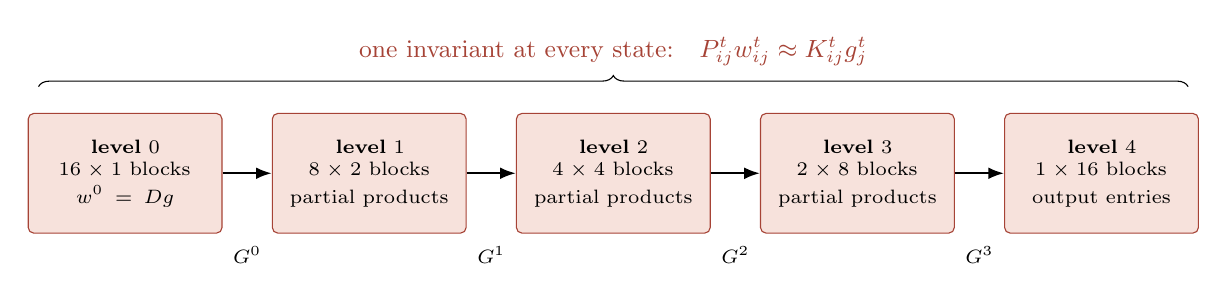
\begin{tikzpicture}[x=1cm,y=1cm]
\node[target] (w0) at (0,0) {\textbf{level $0$}\\$16\times1$ blocks\\[2pt]$w^0=Dg$};
\node[target] (w1) at (3.1,0) {\textbf{level $1$}\\$8\times2$ blocks\\[2pt]partial products};
\node[target] (w2) at (6.2,0) {\textbf{level $2$}\\$4\times4$ blocks\\[2pt]partial products};
\node[target] (w3) at (9.3,0) {\textbf{level $3$}\\$2\times8$ blocks\\[2pt]partial products};
\node[target] (w4) at (12.4,0) {\textbf{level $4$}\\$1\times16$ blocks\\[2pt]output entries};
\draw[flow] (w0)--(w1); \node[font=\scriptsize] at ($(w0)!0.5!(w1)+(0,-1.04)$) {$G^0$};
\draw[flow] (w1)--(w2); \node[font=\scriptsize] at ($(w1)!0.5!(w2)+(0,-1.04)$) {$G^1$};
\draw[flow] (w2)--(w3); \node[font=\scriptsize] at ($(w2)!0.5!(w3)+(0,-1.04)$) {$G^2$};
\draw[flow] (w3)--(w4); \node[font=\scriptsize] at ($(w3)!0.5!(w4)+(0,-1.04)$) {$G^3$};
\draw[decorate,decoration={brace,amplitude=4pt}] (-1.1,1.10)--(13.5,1.10);
\node[font=\small,text=targetred] at (6.2,1.55) {one invariant at every state:\quad $P_{ij}^tw_{ij}^t\approx K_{ij}^tg_j^t$};
\end{tikzpicture}
\caption{The target-only online sweep for $N=16$.  The geometry is identical to the target half of Figure~\ref{fig:original-pipeline}; the difference is that output partial products now exist from the first step.  The factors $G^2,G^3,U^4$ are shared with the original algorithm, while $D,G^0,G^1$ replace its entire source-and-middle prefix in this example.}
\label{fig:target-only-pipeline}
\end{figure}

The formulas for $P^0$ and $D$ explain the online meaning; they are \emph{not} a recommendation to read and normalize all full columns.  The implemented construction obtains $D$ and the coarse transfers from a balanced middle seed, entirely offline and without additional entry accesses.

\subsection{Constructing the coarse target factors by downward QR}
\label{sec:qr-descent}

Write the represented middle blocks as
\[
 \widetilde K_{ij}^{h}=P_{ij}^{h}W_{ij}^{h},
 \qquad W_{ij}^{h}=C_{ij}^{h}(Q_{ij}^{h})^*.
\]
More generally, suppose level $\ell+1$ is represented as $\widetilde K_{ij}^{\ell+1}=P_{ij}^{\ell+1}W_{ij}^{\ell+1}$, with orthonormal columns in each $P$.  We derive the coarser level $\ell$ without forming a tall complementary block.

For a coarse slot $(i,j)$, put $\jd=\lfloor j/2\rfloor$.  Let $S_j$ select the $2^\ell$ columns of the fine band $B_{\jd}^{L-\ell-1}$ belonging to its child $B_j^{L-\ell}$: the first half for even $j$, the second for odd $j$.  The two relevant row children are $2i$ and $2i+1$.  Form the small stacked coefficient matrix and factor it:
\[
 \mathcal U_{ij}^{\ell}:=
 \begin{bmatrix}
 W_{2i,\jd}^{\ell+1}S_j\\[2pt]
 W_{2i+1,\jd}^{\ell+1}S_j
 \end{bmatrix}
 \in\C^{2\rho_{\ell+1}\times2^\ell},
 \qquad
 \mathcal U_{ij}^{\ell}\approx\mathcal Q_{ij}^{\ell}W_{ij}^{\ell},
 \tag{15}\label{eq:small-QR}
\]
where $\mathcal Q$ has orthonormal columns.  The implementation uses reduced, column-pivoted QR; pivoting chooses the local basis, and $W=\mathcal Q^*\mathcal U$ (with truncation when requested).  An SVD could be used instead.  The new output basis and represented coarse block are
\[
 P_{ij}^{\ell}:=
 \begin{bmatrix}P_{2i,\jd}^{\ell+1}&0\\0&P_{2i+1,\jd}^{\ell+1}\end{bmatrix}
 \mathcal Q_{ij}^{\ell},
 \qquad
 \widetilde K_{ij}^{\ell}=P_{ij}^{\ell}W_{ij}^{\ell}.
 \tag{16}\label{eq:coarse-basis}
\]
This follows by direct substitution into the vertical block identity.  If the small factorization is exact, the represented coarse block is exact; if it is truncated, the error is explicit in \eqref{eq:small-QR}.

The tall product in \eqref{eq:coarse-basis} never needs to be formed.  For an online destination $(i',j')$ at level $\ell+1$, let $c=i'-2\lfloor i'/2\rfloor\in\{0,1\}$ select its half of the rows of $\mathcal Q$.  Then the transfer from \eqref{eq:G-definition} reduces to
\[
 \boxed{\quad G_{i'j'}^{\ell}=
 \begin{bmatrix}
 (\mathcal Q_{i,2j'}^{\ell})_c&(\mathcal Q_{i,2j'+1}^{\ell})_c
 \end{bmatrix},\quad}
 \tag{17}\label{eq:qr-transfer}
\]
where $(\cdot)_c$ selects the top or bottom row half.  Repeating \eqref{eq:small-QR}--\eqref{eq:qr-transfer} for $\ell=h-1,\dots,0$ produces all coarse online transfers.  At level $0$, only $D=W^0$ and the small transfers are stored; the full-column bases remain implicit.

\begin{figure}[htbp]
\centering
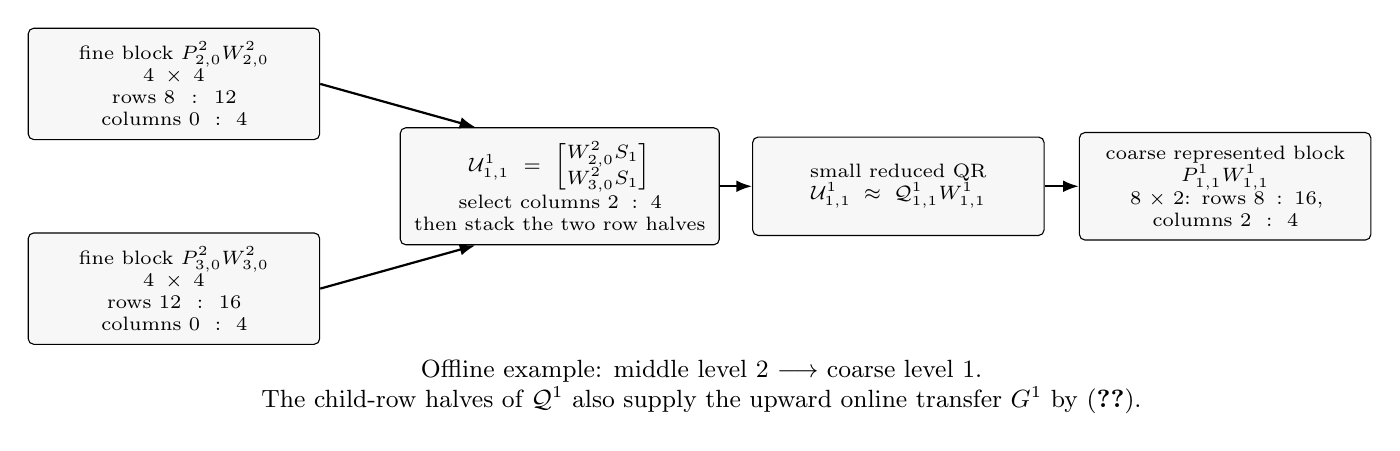
\begin{tikzpicture}[x=1cm,y=1cm,node distance=0.8cm]
\node[construction] (top) at (0,1.20) {fine block $P_{2,0}^2W_{2,0}^2$\\$4\times4$\\rows $8:12$\\columns $0:4$};
\node[construction] (bottom) at (0,-1.40) {fine block $P_{3,0}^2W_{3,0}^2$\\$4\times4$\\rows $12:16$\\columns $0:4$};
\node[construction,text width=3.7cm] (stack) at (4.9,-0.1) {$\mathcal U_{1,1}^1=\begin{bmatrix}W_{2,0}^2S_1\\W_{3,0}^2S_1\end{bmatrix}$\\select columns $2:4$\\then stack the two row halves};
\node[construction] (qr) at (9.2,-0.1) {small reduced QR\\$\mathcal U_{1,1}^1\approx\mathcal Q_{1,1}^1W_{1,1}^1$};
\node[construction] (coarse) at (13.35,-0.1) {coarse represented block\\$P_{1,1}^1W_{1,1}^1$\\$8\times2$: rows $8:16$, columns $2:4$};
\draw[flow] (top.east)--(stack.145);
\draw[flow] (bottom.east)--(stack.215);
\draw[flow] (stack)--(qr);
\draw[flow] (qr)--(coarse);
\node[font=\small,align=center] at (6.7,-2.65) {Offline example: middle level $2$ $\longrightarrow$ coarse level $1$.\\The child-row halves of $\mathcal Q^1$ also supply the upward online transfer $G^1$ by \eqref{eq:qr-transfer}.};
\end{tikzpicture}
\caption{One downward construction step with exact $16\times16$ coordinates.  Here $i=j=1$, so $\jd=0$ and $S_1$ selects the second two columns, $2:4$, of the parent band $0:4$.  The two fine $4\times4$ blocks determine the coarse $8\times2$ block through a small coefficient QR; no large basis matrix product is formed.  This is the offline counterpart of the two-way matrix geometry in Figure~\ref{fig:two-two}.}
\label{fig:qr-example}
\end{figure}

For exact data, induction gives an exact factorization of the represented matrix $\widetilde K$.  With an approximate middle seed, the online sweep represents that seed's approximation, plus any later truncations; it does not silently restore the discarded part of $K$.

At level $\ell$, the small matrix in \eqref{eq:small-QR} has $O(r)$ rows and $2^\ell$ columns.  All $N$ local factorizations at that level cost $O(Nr^22^\ell)$, so
\[
 \sum_{\ell=0}^{h-1}O(Nr^22^\ell)=O(Nr^22^h)=O(N^{3/2}r^2).
 \tag{18}\label{eq:qr-cost}
\]
No entries of $K$ are read in this descent.  Together with the middle seed and the usual upward target recursion, this matches the original construction's asymptotic order for fixed $r$; the seed-specific $O(N^{1/2}C_K(N))$ term remains when black-box products are used.

\subsection{Application and storage have the same asymptotic order}

There are $N$ destination slots per level.  A local transfer has size $\rho_{\ell+1}\times(\rho_a+\rho_b)$, so one level costs $O(N\rho_{\ell+1}\rho_\ell)=O(Nr^2)$, whether it is a source or target transfer.  Both organizations therefore have online cost and sparse-factor storage
\[
 O\!\left(N\sum_{\ell=0}^{L-1}\rho_{\ell+1}\rho_\ell\right)
 =O(Nr^2L)=O(Nr^2\log N),
 \tag{19}\label{eq:online-cost}
\]
which is $O(N\log N)$ for fixed $r$.  A level's temporary state has only $N\rho_\ell\le Nr$ coefficients.  The original form additionally has its middle coupling, and the target-only form its $O(N)$ diagonal initialization; neither changes the order.  The improvement is one coordinate meaning and a smaller online organizational constant, not a new asymptotic rate.

\section{What the implementation and run established}
\label{sec:numerics}

The supplied Python implementation \cite{Numerical} compared the original source--middle--target application with the middle-seeded target-only QR construction.  It used packed slot arrays and the same transfer-application loop for both methods.  This section first reports those existing experiments; Section~\ref{sec:idbfbench} gives the new IDBF implementation and its separate measurements.

\paragraph{Controlled comparison.}  Both branches received exactly the same local middle SVDs and the same upper target factors.  The test matrix was
\[
 K=\frac1{\sqrt{Nr}}AB^*,\qquad A,B\in\C^{N\times r},\qquad r=4,
\]
with reproducible independent standard complex Gaussian entries.  Because $K$ has global rank at most four, every complementary block also has exact rank at most four.  Thus both algorithms had to represent the same operator to roundoff before their speeds were compared.  BLAS/OpenMP was limited to one thread, and reported times were medians over repeated batches.

\paragraph{Correctness.}  On several random complex vectors at $N=16,64$, both outputs were compared with each other and with the exact product $Kg$.  Relative residuals in the supplied final run lay between $8\times10^{-16}$ and $1.8\times10^{-15}$.  The $N=256$ timing check had mutual relative error $1.50\times10^{-15}$.  Correctness was therefore achieved to numerical precision for these deliberately exact-low-rank tests.

\paragraph{Application time.}  Table~\ref{tab:timings} reproduces the supplied final-run application medians.  The target-only version was about $2$--$4\%$ faster: a small but consistent improvement, not an asymptotic one.  The middle map is cheap relative to the $O(Nr^2)$ transfer work at each level, so a large online gain should not be expected.

\begin{table}[htbp]
\centering
\caption{One complete matrix--vector product after offline construction (supplied final run; lower time is better).}
\label{tab:timings}
\begin{tabular}{rcccr}
\toprule
$N$ & original source $+M^h$ ($\mu$s) & target-only ($\mu$s) & original/target & mutual error\\
\midrule
16  & 1.051 & 1.013 & 1.038 & $6.62\times10^{-16}$\\
64  & 2.241 & 2.185 & 1.025 & $1.06\times10^{-15}$\\
256 & 6.968 & 6.837 & 1.019 & $1.50\times10^{-15}$\\
\bottomrule
\end{tabular}
\end{table}

The unshared target-QR construction branch was about $1.7$ times faster than the source-basis branch in that implementation, despite the same $O(N^{3/2}r^2)$ order.  This is a constant-factor comparison of the branches after the shared seed.  Adding the shared literal-SVD seed and common upper construction reduced the whole-setup difference to $17$--$21\%$; it would be incorrect to call the entire factorization $1.7$ times faster.  At $N=256$, the structural online-entry counts were $44{,}544$ and $43{,}520$, respectively.

For this report, the same two scripts were rerun with one BLAS/OpenMP thread.  The correctness checks passed again with residuals of order $10^{-15}$, the target-only application remained slightly faster, and the unshared construction ratios were $1.66$, $1.71$, and $1.75$ at $N=16,64,256$.  Absolute microsecond timings vary by machine and library build and are not treated as portable measurements.

These experiments do not establish a universal stability theorem, behavior for nontrivial approximation tolerances, or superiority of a production sparse-kernel implementation.  The shared test seed used literal block SVDs, not the paper's randomized seed.  The supported conclusion is precise: the alternative was implemented and run, achieved correctness and slightly lower runtime in these tests, and retained the same asymptotic complexity.

\section{Extension to interpolative decomposition butterfly factorization}
\label{sec:idbf}

The later IDBF algorithm of Pang, Ho, and Yang \cite{IDBF} uses the same complementary geometry but different local compressions.  Its leaf--root complementary skeletonization and recursive matrix splitting proceed from both extremes toward a middle factor:
\[
 K\approx U^LU^{L-1}\cdots U^hS^hV^h\cdots V^{L-1}V^L .
\]
During application, input/interpolation coordinates consequently precede middle skeleton data and output interpolation.  The same two-meaning organization appears, although the factors are interpolative rather than the SVD-based factors above.

A target-only, single-invariant counterpart can be conceived by replacing orthonormal output projections with \textbf{column interpolative decompositions} (cIDs).  A cID of a tall matrix $B$ is
\[
 B\approx B[:,q]V,
 \tag{20}\label{eq:cid}
\]
where $q$ selects a small set of columns and $V$ interpolates all columns from them.  IDBF's sampled cID applies rank-revealing QR to $O(k)$ sampled rows, avoiding construction of the other rows.

Write $N=n_02^L$ with leaf size $n_0=O(1)$; this is the minor generalization of Section~\ref{sec:blocks} used by IDBF.  The key choice is an output basis consisting of original matrix columns restricted to the current row node:
\[
 P_{ij}^{\ell}=K[A_i^\ell,q_{ij}^{\ell}],
 \tag{21}\label{eq:id-basis}
\]
where $q_{ij}^{\ell}$ is a short list of global column indices inside $B_j^{L-\ell}$.  The online state again obeys the one invariant $P_{ij}^{\ell}w_{ij}^{\ell}\approx K_{ij}^{\ell}g_j^{\ell}$.

For the transfer $\ell\to\ell+1$, use the same two parent slots $a,b$ and row restriction $R_{i'}$ as in Figure~\ref{fig:two-two}.  Instead of projecting onto a new orthonormal basis, compute a cID of the candidate matrix
\[
 \mathcal B_{i'j'}^{\ell}:=
 \begin{bmatrix}R_{i'}P_a^\ell&R_{i'}P_b^\ell\end{bmatrix}
 \approx P_{i'j'}^{\ell+1}G_{i'j'}^{\ell},
 \qquad
 P_{i'j'}^{\ell+1}:=(\mathcal B_{i'j'})[:,p].
 \tag{22}\label{eq:id-transfer}
\]
The online update remains $w_{i'j'}^{\ell+1}=G_{i'j'}^{\ell}[w_a^\ell;w_b^\ell]$.  Substitution, exactly as in \eqref{eq:target-proof}, shows that restriction and band addition are exact and the cID residual is the only new local error.  Since the candidates are original columns restricted to the child, the selected columns also satisfy \eqref{eq:id-basis}; the new index list is a subset of the two parent lists.

This choice has an important offline consequence.  Sampling $O(k)$ rows of $\mathcal B$ means sampling entries of the original $K$ at known row and column indices.  There are only $O(k)$ candidate columns, so a sampled cID costs $O(k^3)$ operations per slot, without forming a tall basis, a wide coefficient matrix, or a middle seed.  One can therefore construct the factors directly from the row root toward the row leaves, preserving IDBF's orders $O(k^3N\log N/n_0)$ for construction and $O(k^2N\log N/n_0)$ for storage and application under the same sampled-ID assumptions.

Initialization is also compatible with the invariant.  When $n_0\le k$, retain each full column leaf at level $0$ and set $w_{0j}^0=g_j^0$; this is exact and is simply an input permutation, with no tall basis stored.  If $n_0>k$, an initial sampled cID reduces the leaf width.  At level $L$, the output blocks have constant height $n_0$, so their small bases can be formed explicitly and applied.

\begin{center}
\fcolorbox{black!35}{black!4}{\parbox{0.94\textwidth}{
Thus the target-only idea applies to the more recent IDBF algorithm as well: column IDs replace the projections, and the entire online sweep carries output partial products in original-column bases.  Section~\ref{sec:idbfbench} makes this concrete in a controlled local-ID prototype and compares the two online organizations.  The mathematical construction above explains the optimized sampling route; it must be distinguished from the prototype's deliberately simpler entry-access pattern.
}}
\end{center}

The qualifications mirror those of sampled IDBF itself: sampled rows must reveal the range, retained ranks and interpolation coefficients must be controlled, and local residuals accumulate through levels.  The operation count alone is not an unconditional global error bound.

\section{IDBF implementation and controlled benchmarks}
\label{sec:idbfbench}

Section~\ref{sec:idbf} gave the one-sided mathematical construction.  A new Python/NumPy/SciPy prototype implements both online organizations, using only the attached IDBF paper and the structure of the earlier butterfly comparison \cite{IDBF,IDBFCode}.  This is a small, controlled realization of the two-sided factorization, not a translation of the authors' optimized MATLAB code.

\subsection{The normalization that was implemented}
\label{sec:idbf-normalization}

The two applications receive the same middle data.  For each middle block, an rID followed by a CID gives the leaf--root complementary skeletonization
\[
 K_{ij}^{h}\simeq U_{ij}R_{ij},\qquad
 R_{ij}=K[r_{ij},B_j^h],\qquad
 R_{ij}\simeq S_{ij}V_{ij},\qquad
 S_{ij}=R_{ij}[:,q_{ij}].
\]
Set $P_{ij}^{h}=U_{ij}S_{ij}$, $C_{ij}=S_{ij}^{-1}$, and $W_{ij}^{h}=V_{ij}$.  Then
\[
 K_{ij}^{h}\simeq P_{ij}^{h}C_{ij}R_{ij}
 =P_{ij}^{h}W_{ij}^{h}.
 \tag{23}\label{eq:id-normalized-seed}
\]
Here $P_{ij}^{h}$ is also $K[A_i^h,q_{ij}]$ up to the local ID residuals: it consists of selected original columns, exactly as required by \eqref{eq:id-basis}.  The small inverse $C_{ij}$ is formed offline; no inverse is computed or applied online.  This normalization writes the paper's $U S V$ factors as $P C R$ with $P=US$ and $C=S^{-1}$.  Its convenience is that $C Rg$ gives precisely the target coordinates for the shared output basis $P$.

In the paper-style application, a source slot holds the selected-row coordinates $z_{ij}^{\ell}=R_{ij}^{\ell}g_j^{\ell}$.  At level $0$, each full-column leaf keeps its scalar input entry exactly.  For $a,b$ and row restriction as before, a new level satisfies
\[
 z_{i'j'}^{\ell+1}=F_{i'j'}^{\ell}
 \begin{bmatrix}z_a^{\ell}\\z_b^{\ell}\end{bmatrix},
 \qquad
 F_{i'j'}^{\ell}:=R_{i'j'}^{\ell+1}
 \begin{bmatrix}R_a^{\ell}&0\\0&R_b^{\ell}\end{bmatrix}^{+},
 \tag{24}\label{eq:id-source-transfer}
\]
where $^{+}$ is the small Moore--Penrose pseudoinverse used only in the prototype's offline construction.  Substitution makes the relation to $R_{ij}^{\ell}g_j^{\ell}$ immediate whenever the row-basis relation is exact; local interpolation residuals give the approximate version.  At level $h$, multiply by $C_{ij}$, and then continue with the common upper target factors.

The alternative instead computes target partial products $($including $W^hg$$)$ at every level.  Its lower factors use the original-column CID transfer \eqref{eq:id-transfer}; both algorithms use the same upper CIDs and terminal output blocks.  To share the middle basis without altering the interpolation direction, the final lower transfer solves
\[
 P_{i'j'}^{h}G_{i'j'}^{h-1}\simeq\mathcal B_{i'j'}^{h-1}.
 \tag{25}\label{eq:id-middle-align}
\]
Afterwards, both applications perform $G$ updates and terminal multiplications in precisely the same output coordinates.  Schematically, the first application is
\[
 g\longrightarrow z^0\longrightarrow F^1,\dots,F^h
 \longrightarrow C^h\longrightarrow G^h,\dots,G^{L-1},
\]
whereas the target-only application follows one $G$ chain from its exact scalar initialization through the same upper levels.  Neither application accesses $K$ or stores the tall selected-column bases except for constant-height terminal blocks.  A local online transfer or middle coupling contains $O(k^2)$ coefficients, so both online forms retain the order $O(k^2N\log N/n_0)$ for storage and application, with the target partial-product invariant of Section~\ref{sec:idbf} throughout the second.

\subsection{Comparison protocol and scope}
\label{sec:idbf-protocol}

The tests use the same reproducible complex Gaussian model $K=AB^*/\sqrt{Nr}$ as in Section~\ref{sec:numerics}, with $N=16,64,256$ and exact global rank $r=4$.  The leaf size is $n_0=1$ and the local rank cap is $\min(k,N/2^{\ell},2^{\ell})$.  These choices make every complementary block exactly rank at most four and avoid confounding an application-speed comparison with an approximation-tolerance difference.  Reported timings use one BLAS/OpenMP thread, seven $0.25$-second application batches, and medians of their per-call times.  Construction timings use five $0.08$-second batches.  Both methods use the same two-sided middle seed, the same upper factors, and the same destination-slot update implementation.

\begin{center}
\fcolorbox{black!35}{black!4}{\parbox{0.94\textwidth}{
\textbf{Construction-scope caveat.}  The prototype uses deterministic rank-revealing QR and small least-squares calculations on visible local data as a mathematical oracle.  It does not implement the paper's carefully organized sampled-entry LRCS/MSCS construction.  Its branch and full-setup times therefore compare these prototype implementations only: they do not measure or establish the paper's $O(N\log N)$ construction scaling, and they must not be used to claim a threefold speedup for an optimized IDBF factorization.
}}
\end{center}

\subsection{Correctness and measured results}

Correctness was tested at $N=16,64,256$ in three independent ways.  Four random complex vectors at each size gave relative errors against $Kg$ of $1.13$--$2.16\times10^{-15}$ for the original-style form and $1.23$--$1.63\times10^{-15}$ for target-only.  Applying the full factorizations to all coordinate vectors gave maximum original-style relative operator errors of $1.56\times10^{-15}$, with target-only checked against $K$ on every coordinate vector as well.  Second, direct inspection of the original-style selected-row coordinates and the target-only middle products gave worst errors $5.00\times10^{-15}$ and $5.94\times10^{-15}$, respectively.  Third, the target partial-product identity was checked separately at every slot and every level, with worst error $1.40\times10^{-14}$.  All assertions passed; these are roundoff-level checks for the exact-rank oracle, not a general sampled-ID stability theorem.

Table~\ref{tab:idbf-app} reports the final application run.  The source-to-middle-to-target form takes between $1.068$ and $1.123$ times as long as the target-only form.  Thus the latter has roughly $7$--$12\%$ lower runtime across these sizes, a modest constant-factor gain qualitatively similar to the earlier SVD experiment.  At $N=256$, its structural online-entry count is $43{,}264$ rather than $47{,}360$.  The omitted middle coupling and source-coordinate stage explain the qualitative reduction; the common $O(Nk^2)$ transfer work remains.

\begin{table}[htbp]
\centering
\caption{One complete IDBF matrix--vector product after offline construction (final prototype run; lower time is better).}
\label{tab:idbf-app}
\begin{tabular}{rcccr}
\toprule
$N$ & original source $+C^h$ ($\mu$s) & target-only ($\mu$s) & original/target & mutual error\\
\midrule
16  &   98.237 &   87.477 & 1.123 & $1.27\times10^{-15}$\\
64  &  534.625 &  491.678 & 1.087 & $1.59\times10^{-15}$\\
256 & 2670.066 & 2500.892 & 1.068 & $2.56\times10^{-15}$\\
\bottomrule
\end{tabular}
\end{table}

\begin{table}[htbp]
\centering
\caption{Visible-entry prototype construction timings, in milliseconds, subject to the scope caveat above.  ``Full'' adds the shared two-sided-ID seed and shared upper CIDs to the unshared branch timings.}
\label{tab:idbf-build}
\small
\setlength{\tabcolsep}{4.2pt}
\begin{tabular}{rccccc}
\toprule
$N$ & source branch & target branch & branch ratio & original full & target full\\
\midrule
16  &  0.789 &  0.305 & 2.588 &  1.690 &  1.206\\
64  &  5.707 &  1.824 & 3.129 & 11.532 &  7.649\\
256 & 38.872 & 12.550 & 3.097 & 68.601 & 42.279\\
\bottomrule
\end{tabular}
\end{table}

Table~\ref{tab:idbf-build} separates the unshared interpolation branches from the shared middle seed and upper construction.  The source/target ratios for the full visible-entry prototype setup are $1.40$, $1.51$, and $1.62$, respectively.  These numbers concern concrete small-matrix code constants, memory layout, pseudoinverses and interpolation solves, not a new asymptotic construction result.  Repeating the complete driver reproduced the correctness results and closely reproduced the application ratios (about $1.07$--$1.12$ in three runs).

The supported conclusion therefore extends the earlier one in a qualified but concrete way: a two-sided IDBF online organization and a target-only counterpart were implemented in a shared-seed prototype, their invariants and full outputs were verified, and the target-only version used less online time and storage.  Optimized sampled construction, non-exact low-rank truncation behavior, Mock--Chebyshev versus random sampling, and production sparse-kernel performance remain outside the experiment.

\section{Conclusion}

The original butterfly algorithm is understandable through two online statements: source slots store $Q^*g$ for their input bands, then target slots store $P^*Kg$ for their block partial products.  The middle joins them because balanced blocks are the cheapest generic offline seed, not because a vector has already been applied there.  A downward small-QR recursion converts that same seed into a target-only factorization whose single invariant holds at every level.  The implemented comparison supports this simpler organization with roundoff-level correctness, slightly lower measured runtime, and unchanged asymptotic complexity.

For IDBF, original-column interpolation replaces orthonormal projection.  The mathematical construction makes one target invariant possible from the row root to the row leaves.  The new shared-seed prototype implements and verifies both IDBF online organizations; in the controlled exact-rank tests, target-only reduces application time and storage.  The optimized sampled-entry construction of IDBF was not benchmarked, so no corresponding construction-complexity claim is inferred from the prototype timings.


\begin{thebibliography}{9}
\bibitem{BF}
Y.~Li, H.~Yang, E.~R.~Martin, K.~L.~Ho, and L.~Ying,
\emph{Butterfly factorization},
Multiscale Modeling \& Simulation \textbf{13} (2015), no.~2, 714--732.
DOI: \href{https://doi.org/10.1137/15M1007173}{10.1137/15M1007173}.
Sections 2--3 give the middle-level construction and the two recursive factorizations.

\bibitem{IDBF}
Q.~Pang, K.~L.~Ho, and H.~Yang,
\emph{Interpolative decomposition butterfly factorization},
arXiv:1809.10573v2, 2018.
Sections 2.1--2.4 give linear sampled cIDs, leaf--root skeletonization, and recursive matrix splitting.

\bibitem{Numerical}
\emph{Numerical comparison of two butterfly applications: source coordinates with a middle hand-off versus target coordinates throughout}, supplied companion report \texttt{numericalResults.pdf}, with \texttt{butterfly\_algorithms.py} and \texttt{compare\_butterfly.py}.
The two scripts implement the middle-seeded SVD/QR algorithms and their controlled correctness and timing comparison.

\bibitem{IDBFCode}
\emph{Controlled IDBF applications with a shared two-sided interpolative seed}, new prototype in \texttt{results/idbf\_algorithms.py}, with the correctness and timing driver \texttt{results/compare\_idbf.py} and raw results \texttt{results/idbf\_benchmark\_results.json}.  Its documentation distinguishes visible-entry mathematical-oracle construction from optimized sampled-entry IDBF construction.
\end{thebibliography}

\end{document}
